\documentclass{beamer}
\usepackage{textcomp}
\usepackage[ngerman]{babel}
\usepackage[utf8]{inputenc}
\usepackage[T1]{fontenc}
\usepackage{fancybox}
\usepackage{graphicx}
\usepackage{hyperref}
\usepackage{amssymb}
\usepackage{amsmath}
\usepackage{amsthm}
\usepackage{listings}
\usepackage[scaled]{luximono}
\usepackage{tikz}

\tikzset{
  every overlay node/.style={
    draw=white,fill=white,rounded corners,anchor=north west,
  },
}
% Usage:
% \tikzoverlay at (-1cm,-5cm) {content};
% or
% \tikzoverlay[text width=5cm] at (-1cm,-5cm) {content};
\def\tikzoverlay{%
   \tikz[baseline,overlay]\node[every overlay node]
}%

\usetheme{Berlin}
\useoutertheme{infolines}
\usefonttheme{professionalfonts}
\usecolortheme{seahorse}
\usecolortheme{rose}

%\setbeamercovered{transparent}
\beamertemplatenavigationsymbolsempty
\setbeamertemplate{footline}[frame number]
\theoremstyle{example}
\newtheorem{ex}{Beispiel}
\renewenvironment{example}{\begin{ex}}{\end{ex}}


\title{Bilder In Weniger Als Tausend Worten}
\subtitle{Girlsday 2012}
\institute{Universit\"at des Saarlandes}
\date{}
\author[A. Neumann]{
	Adrian Neumann
}



\begin{document}
\lstdefinelanguage{cf}{morekeywords={shape,rule,CF,startshape,SQUARE,CIRCLE,TRIANGLE}, sensitive=true}
\lstset{basicstyle=\ttfamily\footnotesize, numbers=left, numberstyle=\tiny, language=cf, tabsize=2}
\frame{\titlepage}

\section{Rechnen}
\begin{frame}{Rechnen}
Manipulation eines Speichers nach festen Regeln\pause
\begin{itemize}
\item Mathe auf Papier\pause
\item Programme in Computern\pause
\item Billiardbälle auf einem Billiardtisch\pause
\end{itemize}
\begin{block}{}\centering
Informatiker untersuchen einfache Regelsysteme mit kompliziertem Verhalten
\end{block}
\end{frame}

\subsection{Beispiel:Game of Life}
\begin{frame}{Beispiel: Game of Life}
\begin{itemize}
\item Speicher: 
  \begin{itemize}
    \item 2D-Gitter\pause
    \item Zellen sind ``lebendig'' (weiß) oder ``tot'' (schwarz)\pause
  \end{itemize}
\item Regeln\pause
  \begin{itemize}
  \item Lebendig $\rightarrow$ Tot: $<2$ oder $>3$ lebendige Nachbarn\pause
  \item Lebendig $\rightarrow$ Lebendig: $2$-$3$ lebendige Nachbarn\pause
  \item Tot $\rightarrow$ Lebendig: 3 lebendige Nachbarn
  \end{itemize}
\end{itemize}\pause
\begin{block}{}\centering
\centering In Game of Life kann ein beliebiger Computer simuliert werden.
\end{block}
\end{frame}

\begin{frame}{Beispiel: Game of Life}
\onslide*<1>{\begin{center}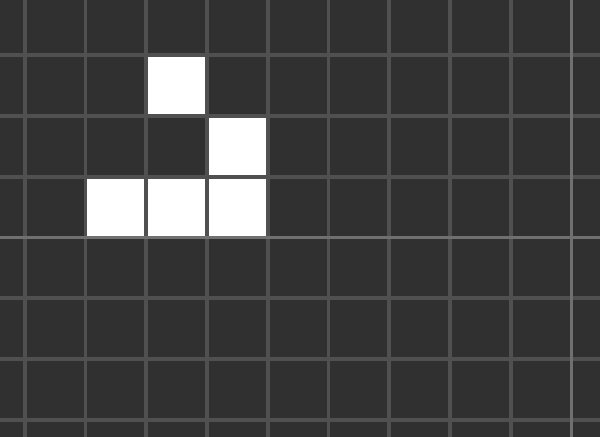
\includegraphics[width=0.8\linewidth]{./images/glider1.png}\end{center}}
\onslide*<2>{\begin{center}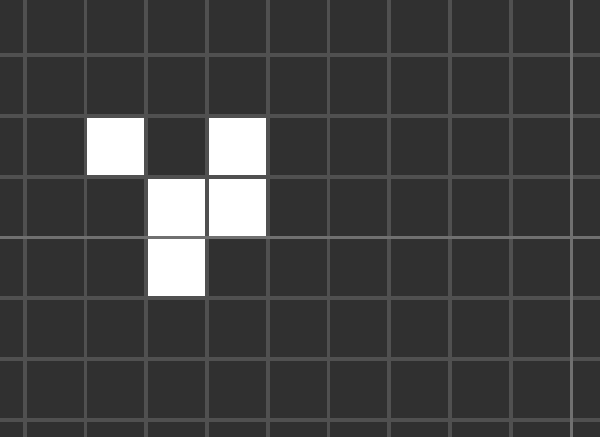
\includegraphics[width=0.8\linewidth]{./images/glider2.png}\end{center}}
\onslide*<3>{\begin{center}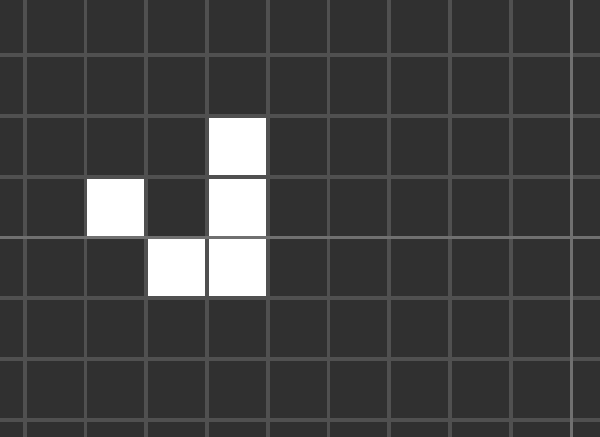
\includegraphics[width=0.8\linewidth]{./images/glider3.png}\end{center}}
\onslide*<4>{\begin{center}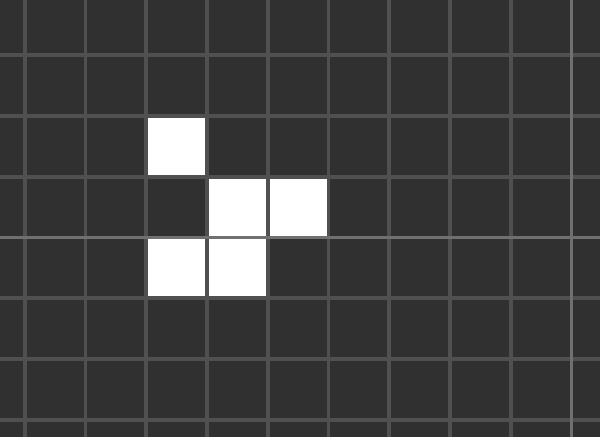
\includegraphics[width=0.8\linewidth]{./images/glider4.png}\end{center}}
\onslide*<5>{\begin{center}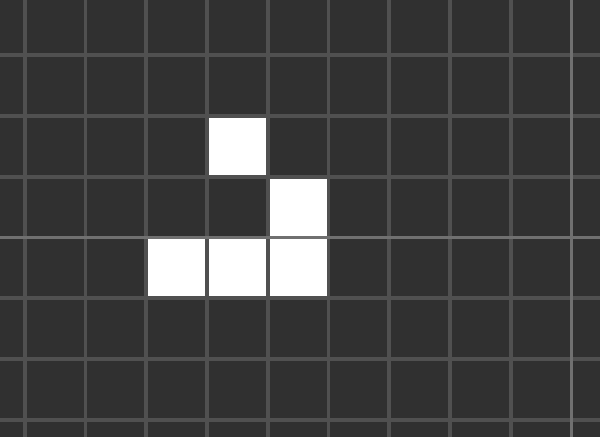
\includegraphics[width=0.8\linewidth]{./images/glider5.png}\end{center}}
\onslide*<6>{\begin{center}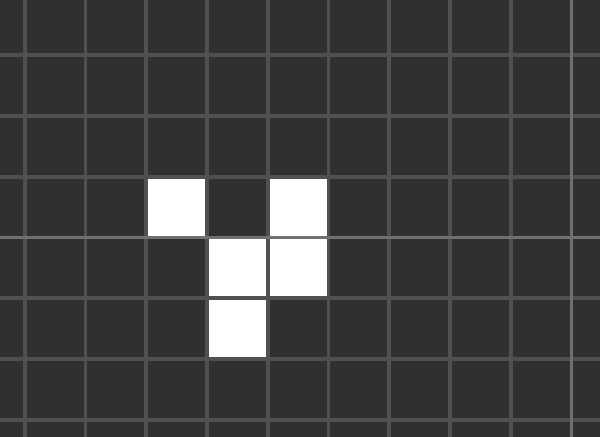
\includegraphics[width=0.8\linewidth]{./images/glider6.png}\end{center}}
\onslide*<7>{\begin{center}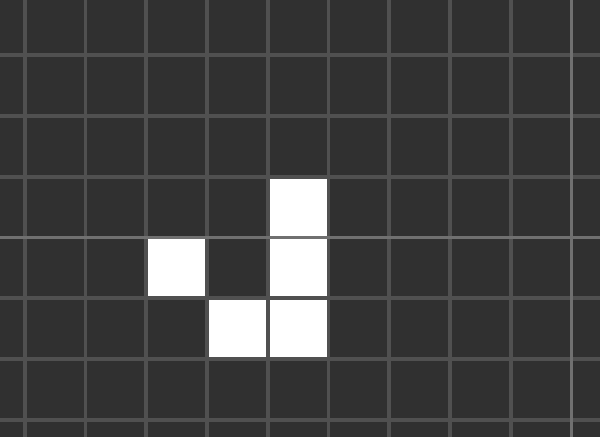
\includegraphics[width=0.8\linewidth]{./images/glider7.png}\end{center}}
\onslide*<8>{\begin{center}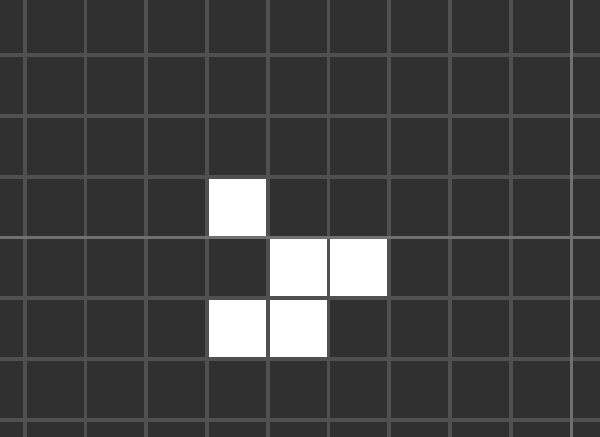
\includegraphics[width=0.8\linewidth]{./images/glider8.png}\end{center}}
\onslide*<9>{\begin{center}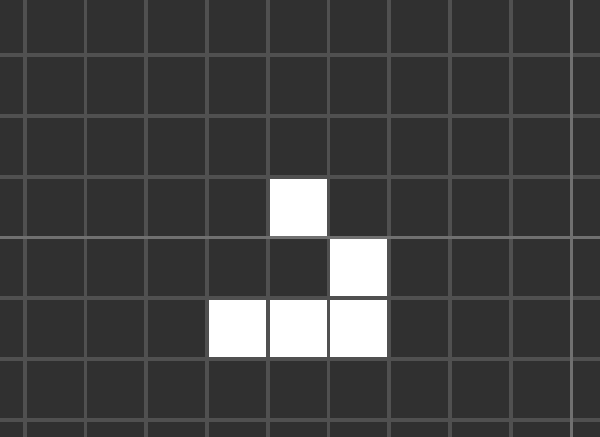
\includegraphics[width=0.8\linewidth]{./images/glider9.png}\end{center}}

\end{frame}

\section{Arbeiten mit ``Sprachen''}
\begin{frame}{Sprache}
  \begin{definition}
    \begin{description}
    \item[Alphabet:] Endliche Menge von ``Buchstaben''
    \item[Wort:] Endliche Sequenz von Buchstaben
    \item[Sprache:] Menge von Wörtern (i.\,d.\,R.\ unendlich)
    \end{description}
  \end{definition}\pause
  \begin{example}
    \begin{description}
    \item[Alphabet:] $\Sigma = \{ (,)\}$
    \item[Wort:] $()(())$ oder $((())$ oder $))(($ \ldots
    \item[Sprache:] $L=\{w | \text{$w$ ist korrekt geklammert}\}$
      $L = \{(),(()),()(),(())(),\ldots\}$
    \end{description}
  \end{example}
\end{frame}

\subsection{Grammatiken}
\begin{frame}{Grammatiken}
  \begin{itemize}
  \item Einfache Regeln zum Beschreiben von Sprachen\pause
  \item ``Grammatik'' wie in der Schule: Irreführend\pause
  \item Zwei Arten von Symbolen:\pause
    \begin{itemize}
    \item Buchstaben (\emph{Terminalzeichen}): hier Kleinbuchstaben $a,b,c$
    \item Platzhalter (\emph{Nichtterminalzeichen}): hier Großbuchstaben $A,B,C$
\pause\par
      Ein Nichtterminalzeichen ist besonders: Das \emph{Startsymbol}\pause
    \end{itemize}
  \item Regeln um Wörter zu erzeugen\pause
  \item Sprache: Menge aller Wörter, die man mit der Grammatik erzeugen kann
  \end{itemize}
\end{frame}

\subsection{Produktionsregeln}
\begin{frame}{Produktionsregeln}
  \begin{itemize}
  \item\onslide<1-> Regeln haben die Form
    \[\text{\textit{String}}_1 \longrightarrow \text{\textit{String}}_2\]
  \item\onslide<2-> Darf linke Seite durch rechte Seite ersetzen
  \item\onslide<3-> Angefangen wird mit dem Startsymbol
  \item\onslide<4-> Prozess ist abgeschlossen, wenn kein Nichtterminal übrig ist
  \end{itemize}
\onslide<5->{
\hspace{2cm} Heute: \emph{Kontextfreie} Grammatiken

\hspace{2cm} \textit{String$_1$} ist genau ein Nichtterminal
}
\end{frame}

\subsection{Beispiel: Klammerausdrücke}
\begin{frame}{Beispiel}
  \begin{itemize}
  \item Schon gesehen: $\Sigma = \{(,)\}$ und  $L = \{ w | \text{$w$ ist korrekt geklammert}\}$\pause
  \item Grammatik:
    \begin{columns}[l]
     \column{2cm}
    \begin{align*}
      S &\rightarrow ()\\
      S &\rightarrow SS\\
      S &\rightarrow (S)
    \end{align*}\pause
     \column{6cm}
     \begin{ex}
       \vspace*{5cm}
       \hspace*{6cm}
     \end{ex}
    \end{columns}
  \end{itemize}
\end{frame}

\begin{frame}{Anwendungen}
  \begin{itemize}
  \item Computerlinguistik\pause
  \item Programmiersprachen\pause
  \item Theoretische Informatik\pause
    \begin{itemize}
    \item Wie ``aufwendig'' ist es festzustellen ob $w\in L$?\pause
    \item Ist $L = \{w | \text{$w$ ist korrekt geklammert}\}$ ``schwieriger'' als $L = \{w | \text{$w$ ist eine wahre Aussage}\}$?\pause
    \item Gibt es Sprachen, für die man gar nicht feststellen kann ob $w\in L$?
    \end{itemize}

  \end{itemize}
\end{frame}


\subsection{Mehr als Buchstaben}
\begin{frame}{Mehr als Buchstaben}
  \begin{itemize}
  \item Besonderes Alphabet\pause
    \begin{itemize}
    \item Geometrische Primitive (Rechteck, Dreieck, Kreis)\pause
    \item Rotationen\pause
    \item Skalierungen\pause
    \item Translationen\pause
    \item Farbveränderungen\pause
    \end{itemize}
  \item Grammatik regelt, wie daraus Bilder erzeugt werden
  \end{itemize}
\end{frame}

\section{Context-Free Art}
\begin{frame}[fragile]{Kompliziertes Beispiel}
\begin{columns}
\onslide<2>\column{4cm}
\footnotesize{
\begin{lstlisting}
CF::Background = [b -1]
startshape T[
  b 1 a -1 sat 1 h 310
]

shape T
rule {
  SQUARE[x .5 y -.05 s 1 .1]
  CIRCLE[x 1.77 y .13 s .5]
  T[r -2.07028 s 0.298966
    a .1 h 90 sat -.3]
  T[x 1 r 45.9297 s .324258
    a .1 sat .1]
  T[x 1.72574 y .806014
    r -48 s .922]
} 
\end{lstlisting}
}
\onslide<1->\column{6cm}
\hfill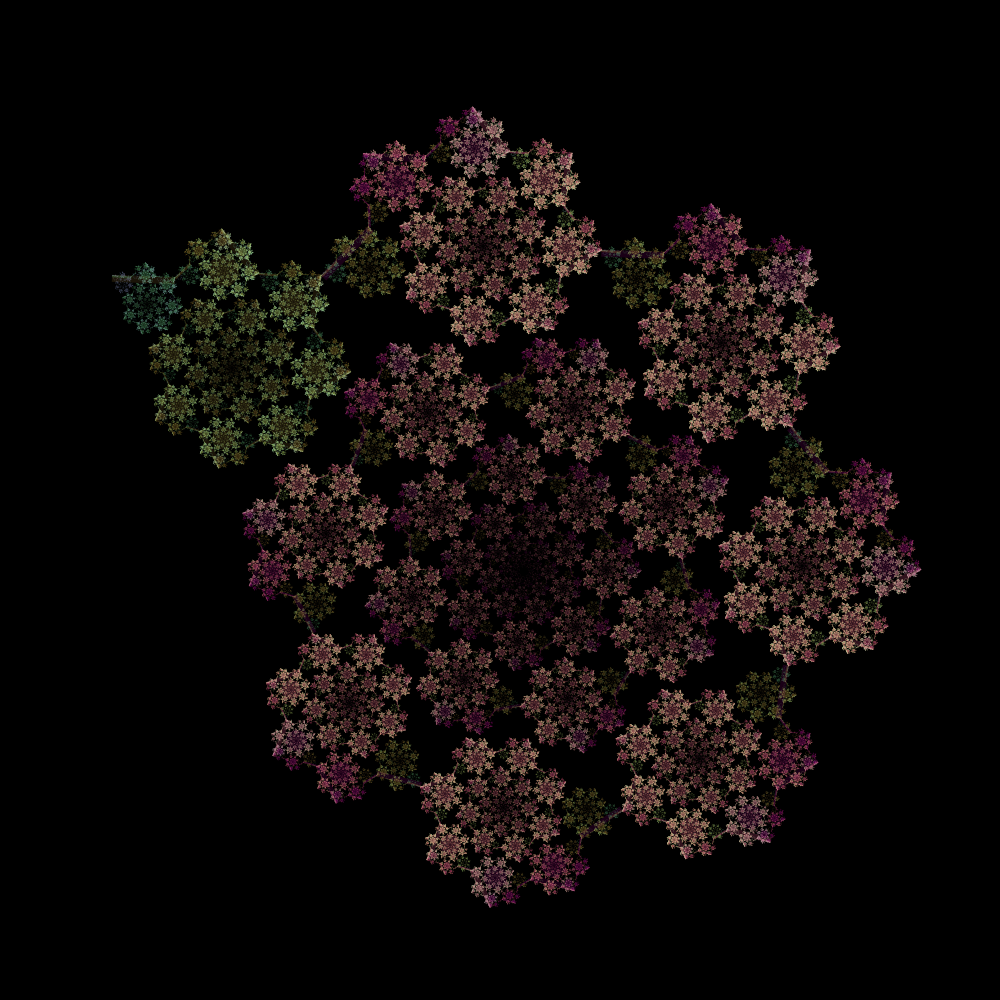
\includegraphics[width=\linewidth]{./images/beispiel.png}
\end{columns}
\tiny
\hfill CC-BY-SA 3.0 zol
\end{frame}

\newsavebox\mybox

\begin{lrbox}{\mybox}
\begin{lstlisting}[name=beispiel]
CF::Background = [b -1]
startshape T[
  b 1 a -1 sat 1 h 310
]
\end{lstlisting}
\end{lrbox}

\begin{frame}[fragile]{Steueranweisungen}

\tikzoverlay at (8cm, 1cm) {
\usebox\mybox
};

Einstellungen für das ganze Bild:\pause
  \begin{itemize}
  \item Beginnen mit \lstinline!CF::!\pause
    \begin{itemize}
    \item Hintergrund: \lstinline!CF::Background!
    \item Minimalgröße der Bildelemente: \lstinline!CF::MinimumSize!
    \item[\vdots]\pause
    \end{itemize}
   \item Im Beispiel: \lstinline!CF::Background = [b -1]!

     Setze \textbf{b}rightness (Helligkeit) auf Minimalwert (=Schwarz).
  \end{itemize}\pause
Startsymbol: 
\begin{itemize}
\item Festgelegt mit \lstinline!startshape!
\end{itemize}
\end{frame}

\begin{frame}{Terminale}
\begin{columns}
\column{5cm}
  Drei verschiedene Terminale:\pause
  \begin{enumerate}
  \item \lstinline!CIRCLE!\pause
  \item \lstinline!SQUARE!\pause
  \item \lstinline!TRIANGLE!\pause
  \end{enumerate}
 \begin{itemize}
 \item Alle haben Seitenlänge 1\pause
 \item Alle werden zentriert an $(0,0)$ gezeichnet
 \end{itemize}
\column{5cm}
 \begin{center}
   \fbox{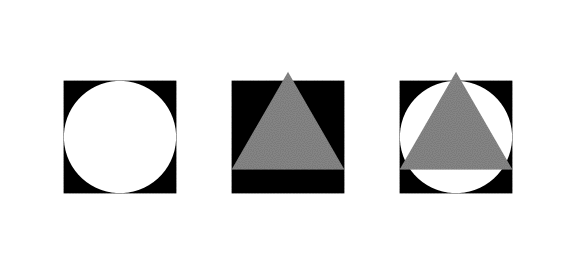
\includegraphics[width=\linewidth]{./images/Shape_demo.png}}\\\bigskip
   Code für dieses Bild: Übung!
 \end{center}
\end{columns}
\end{frame}

\begin{frame}{Terminale: Beispiel}
  \begin{columns}
    \column{3cm}
    \lstinline!startshape CIRCLE[]!
    \begin{center}
    \fbox{
\includegraphics[width=0.8\linewidth]{./images/circle.png}}
    \end{center}
    \column{3cm}
    \lstinline!startshape SQUARE[]!
    \begin{center}
    \fbox{
\includegraphics[width=0.8\linewidth]{./images/square.png}}
    \end{center}
    \column{3cm}
    \lstinline!startshape TRIANGLE[]!
    \begin{center}
    \fbox{
\includegraphics[width=0.8\linewidth]{./images/triangle.png}}
    \end{center}
  \end{columns}
\end{frame}

\begin{lrbox}{\mybox}
\begin{lstlisting}[name=beispiel]
shape T
rule {
  SQUARE[x .5 y -.05 s 1 .1]
  CIRCLE[x 1.77 y .13 s .5]
  T[r -2.07028 s 0.298966
    a .1 h 90 sat -.3]
  T[x 1 r 45.9297 s .324258
    a .1 sat .1]
  T[x 1.72574 y .806014
    r -48 s .922]
} 
\end{lstlisting}
\end{lrbox}


\begin{frame}[fragile]{Nichtterminale}

\tikzoverlay at (7.5cm, 1cm) {
\usebox\mybox
};
  \begin{itemize}
  \item Heißen jetzt \lstinline!shape!\pause
  \item Produktionsregeln: \lstinline!rule {...}! \pause
  \item Im Beispiel
    \begin{itemize}
    \item Nichtterminal: \lstinline!T!\pause
    \item Produktionsregel: Ersetze \lstinline!T! durch
      \begin{itemize}
      \item Ein Viereck \lstinline!SQUARE!
      \item Einen Kreis \lstinline!CIRCLE!
      \item Drei \lstinline!T!
      \end{itemize}
    \end{itemize}\pause
  \item Mehrere \lstinline{rule} können hintereinander stehen.
  \item Welche Regel angewendet wird, wird \emph{zufällig} entschieden\pause
  \item Fertig: Keine Nichtterminale mehr \emph{oder} Alle Bildelemente zu klein
  \end{itemize}
\end{frame}

\begin{frame}[fragile]{Nichtterminale: Beispiel}
\begin{columns}
  \onslide<2>{\column{4cm}
  \lstinputlisting{./code/circle_triangle.cf}}
  \column{4cm}
  \begin{center}
    \fbox{
\includegraphics[width=\linewidth]{./images/circle_triangle.png}}
  \end{center}
\end{columns}
\end{frame}

\begin{frame}{Transformationen}
  \begin{itemize}
  \item Für Matheprofis: Affine Transformation + Farbveränderung\pause
  \item Hinter jedem Element, eckige Klammern mit Anweisungen\pause
  \item Notationsreihenfolge egal. Immer:
    \begin{enumerate}
    \item Verschieben
    \item Rotieren
    \item Skalieren
    \item Reflektieren
    \end{enumerate}\pause
  \item Doppelte Klammern: Reihenfolge zählt\pause
  \item Werden angewendet \emph{nachdem} das Element fertig gezeichnet ist
  \end{itemize}
\end{frame}

\begin{frame}{Transformationen}
\begin{block}{Übersicht: Form}
  \begin{description}
  \item[Verschieben] \lstinline!x!, \lstinline!y! mit einer Zahl dahinter
  \item[Rotieren] \lstinline!r! mit Winkel (Grad) dahinter
  \item[Skalieren] \lstinline!s! mit Skalierungsfaktor dahinter. Zwei Zahlen: x,y-Richtung getrennt skalieren
  \item[Reflektieren] \lstinline!f! (flip) mit Winkel dahinter: Reflektion an Ursprungsgeraden
  \end{description}
\end{block}
\end{frame}

\begin{frame}[fragile]{Transformationen: Beispiel}
  \begin{columns}
    \onslide<1->\column{3cm}
    \lstinputlisting{./code/transformation1.cf}
    \begin{center}
      \fbox{
\includegraphics[width=\linewidth]{./images/transformation1.png}}
    \end{center}
    \onslide<2->\column{3cm}
    \lstinputlisting{./code/transformation2.cf}
    \vspace{-0.75cm}
    \begin{center}
      \fbox{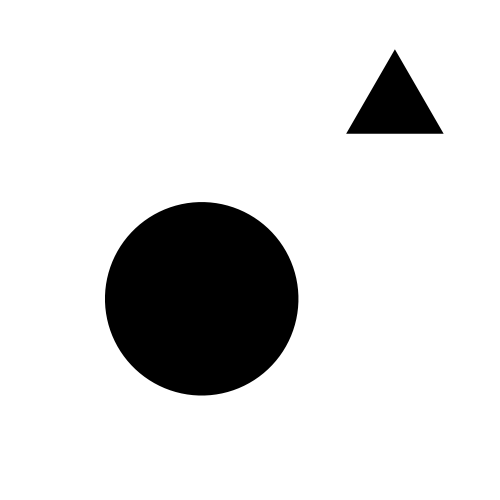
\includegraphics[width=\linewidth]{./images/transformation2.png}}
    \end{center}
    \onslide<3->\column{3cm}
    \lstinputlisting{./code/transformation3.cf}
    \begin{center}
      \fbox{
\includegraphics[width=\linewidth]{./images/transformation3.png}}
    \end{center}
  \end{columns}

\end{frame}

\begin{frame}{Transformationen: Beispiel}
  Skalierungen: nach dem Verschieben angewendet
  \begin{columns}
    \onslide<2->\column{5cm}
    \lstinputlisting{./code/scaling_wrong.cf}
    \begin{center}
      \fbox{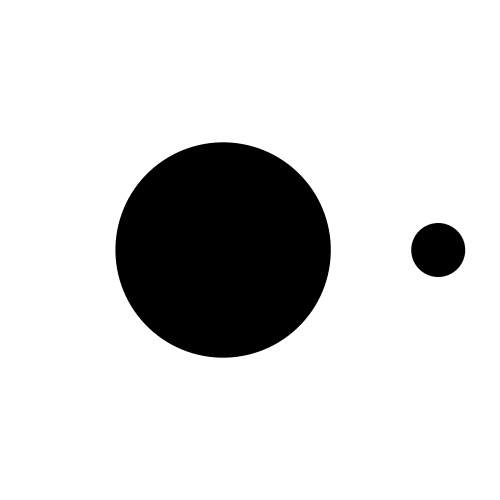
\includegraphics[width=0.7\linewidth]{./images/scaling_wrong.png}}
    \end{center}
    \onslide<3->\column{5cm}
    \lstinputlisting{./code/scaling_right.cf}
    \begin{center}
      \fbox{
\includegraphics[width=0.7\linewidth]{./images/scaling_right.png}}
    \end{center}
  \end{columns}

\end{frame}


\begin{frame}{Transformationen}
\begin{center}
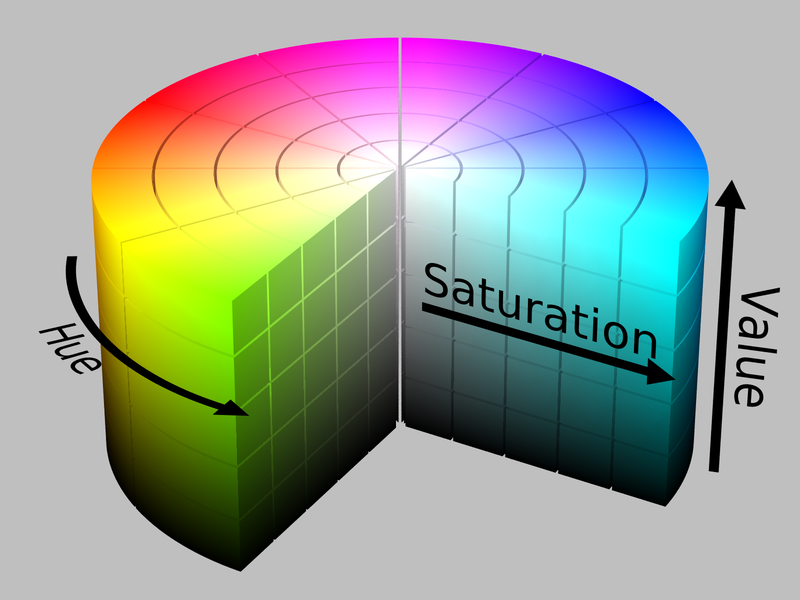
\includegraphics[width=0.7\linewidth]{./images/HSV.png}
\end{center}
\hfill{{\tiny CC-BY-SA Wikipedia User SharkD}}
\end{frame}

\begin{frame}{Transformationen}
\begin{block}{Übersicht: Farbe}
  \begin{description}
  \item[Farbton] \lstinline!h! {\small $n$}, $n\in [0,359]$. 
  \item[Sättigung] \lstinline!sat! {\small $n$}, $n\in [-1,1]$. 
  \item[Helligkeit] \lstinline!b! {\small $n$}, $n\in [-1,1]$.
  \item[Transparenz] \lstinline!a! {\small $n$}, $n\in [-1,1]$.
  \end{description}
\end{block}\pause
Alternative Form: Zwei Zahlen. Zum Beispiel \lstinline!h! {\small $p$ $z$}, $p\in [-1,1]$:\\ Farbton in Richtung $z$ ändern.

\alert{Achtung:} Für \lstinline!CF::Background! werden absolute Werte gesetzt.
\end{frame}

\begin{frame}{Transformationen: Beispiel}
  \begin{columns}
   \onslide<2>\column{6cm}
   \lstinputlisting{./code/transformation5.cf}
   \onslide<1->\column{4cm}
  \begin{center}
    \fbox{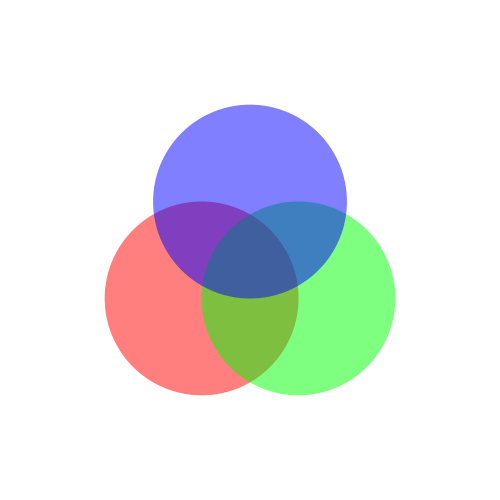
\includegraphics[width=\linewidth]{./images/transformation5.png}}
  \end{center} 
  \end{columns}   
\end{frame}

\begin{frame}{Regeln mit Nichtterminalen}
Transformationen werden \emph{nach} dem Zeichnen angewendet\\
$\longrightarrow$ Können sich ``stapeln''\pause
\begin{columns}
\column{6cm}
\lstinputlisting{./code/rekursion2.cf}\pause
\column{4cm}
\begin{center}
\fbox{
\includegraphics[width=\linewidth]{./images/rekursion2.png}}
\end{center}
\end{columns}\medskip
In jeder Ersetzung $1.2$-Mal heller, $0.8$-Mal kleiner.
\end{frame}

\begin{frame}{Regeln mit Nichtterminalen}
  Besonders verwirrend: Koordinatensystem ändert sich!
\begin{columns}
\onslide<2->\column{6cm}
\lstinputlisting{./code/rekursion1.cf}
\onslide<3->\column{4cm}
\begin{center}
  \fbox{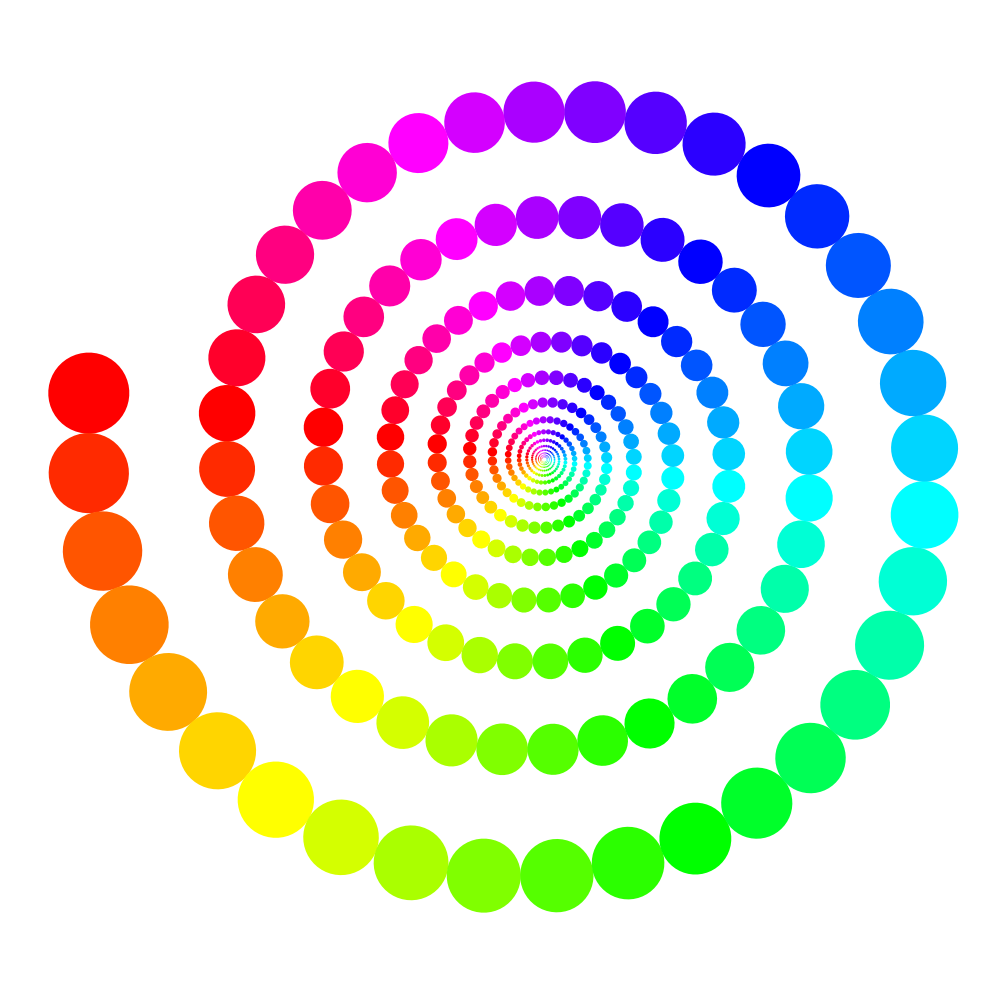
\includegraphics[width=\linewidth]{./images/rekursion1.png}}
\end{center}
\end{columns}\medskip
Verschieben immer nach unten, aber im rotierten Koordinatensystem.
\end{frame}

\begin{frame}{Zufall}
Bei mehreren Produktionsregeln: Zufällige Auswahl. 
  \begin{columns}
    \onslide*<1>{
    \column{5cm}
    \lstinputlisting{./code/randomness2.cf}
    \column{5cm}
    \begin{center}
      \fbox{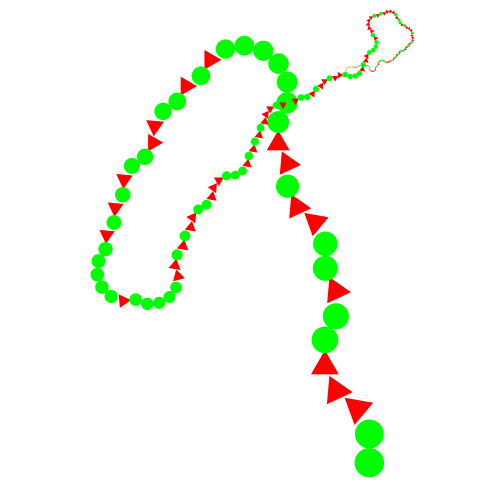
\includegraphics[width=0.9\linewidth]{./images/randomness2.png}}
    \end{center}
    }
    \onslide*<2>{
    \column{5cm}
    \lstinputlisting{./code/randomness3.cf}
    \column{5cm}
    \begin{center}
      \fbox{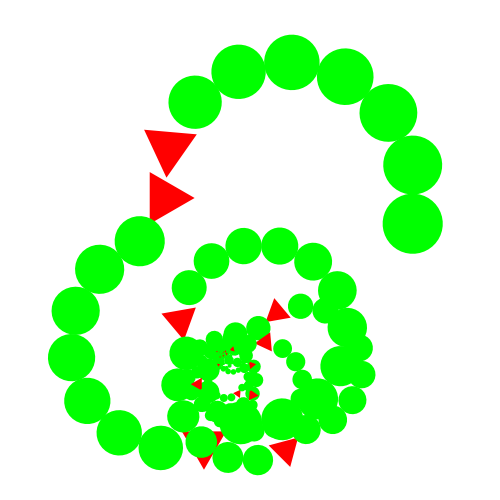
\includegraphics[width=0.9\linewidth]{./images/randomness3.png}}
    \end{center}
  }
  \end{columns}
  
\end{frame}

\begin{frame}{Übungen}
  \begin{columns}
    \column{3cm}
    \fbox{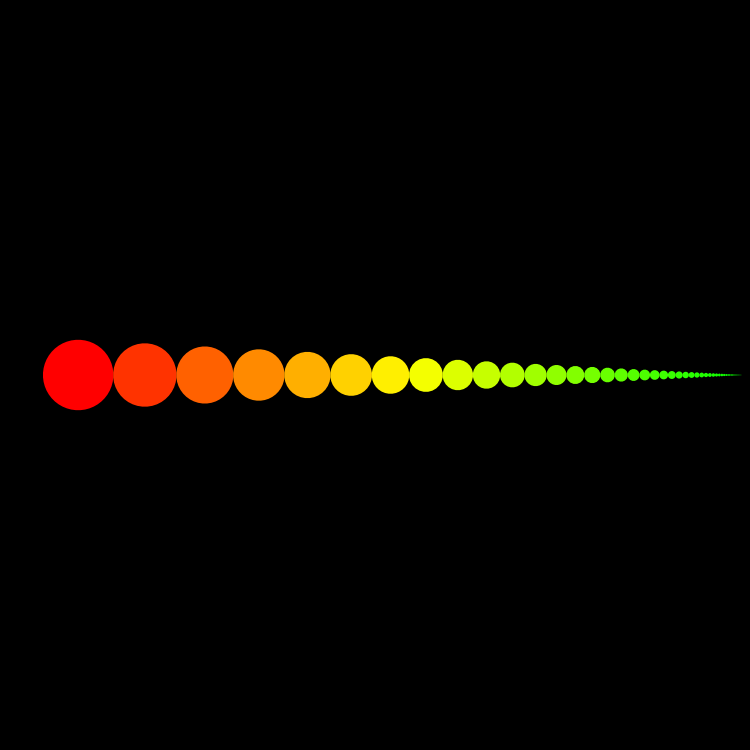
\includegraphics[width=\linewidth]{./images/exercise1.png}}
    \column{3cm}
    \fbox{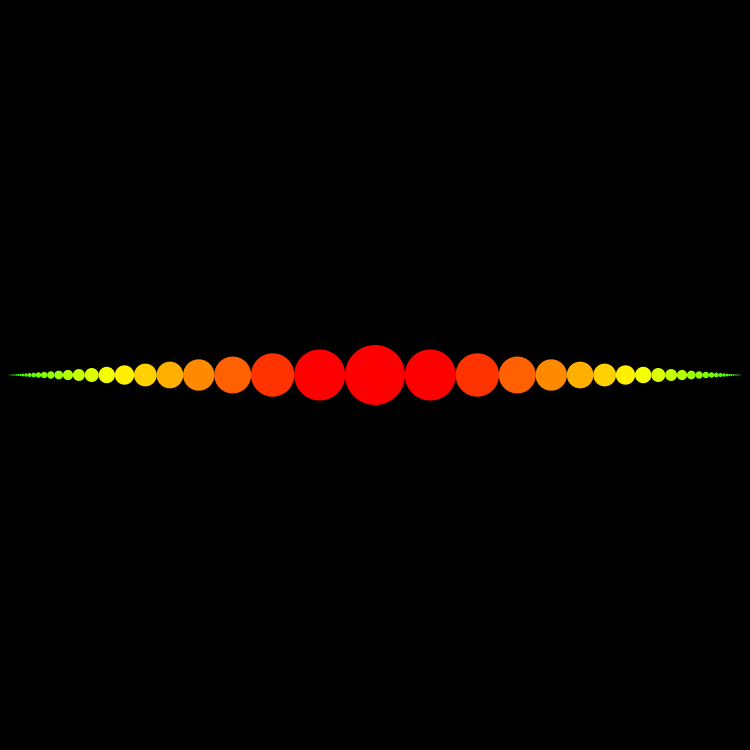
\includegraphics[width=\linewidth]{./images/exercise2.png}}
    \column{3cm}
    \fbox{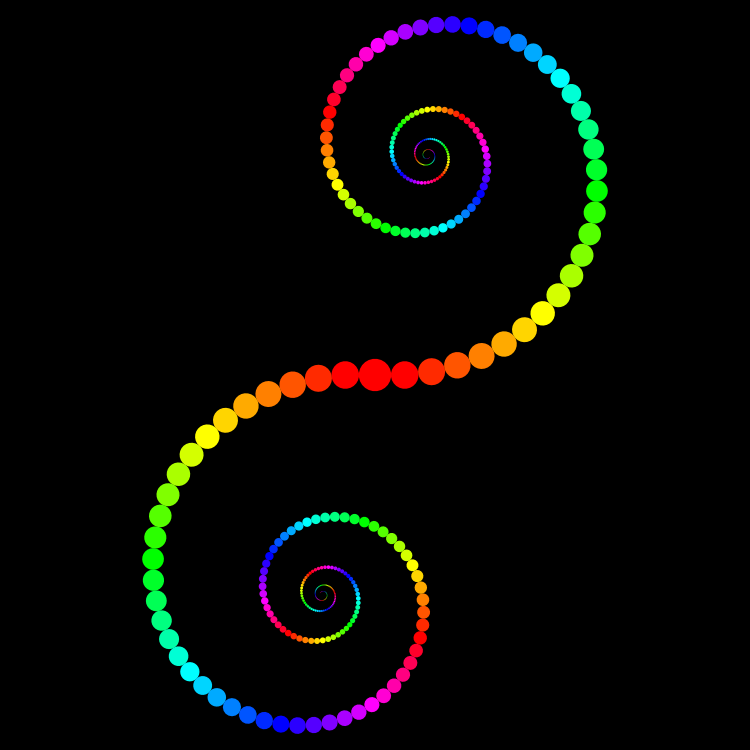
\includegraphics[width=\linewidth]{./images/exercise3.png}}
  \end{columns}
  \begin{columns}
    \column{3cm}
    \fbox{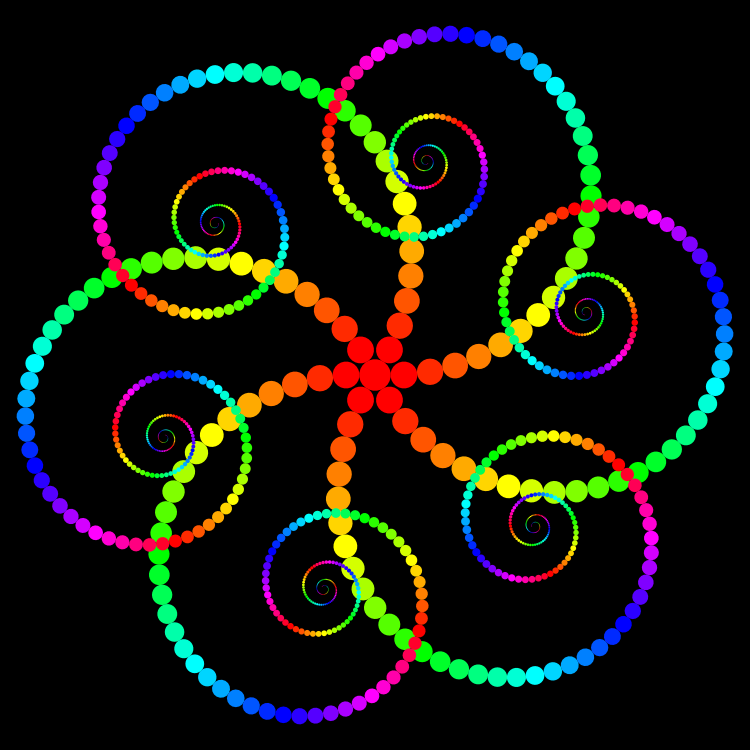
\includegraphics[width=\linewidth]{./images/exercise4.png}}
    \column{3cm}
    \fbox{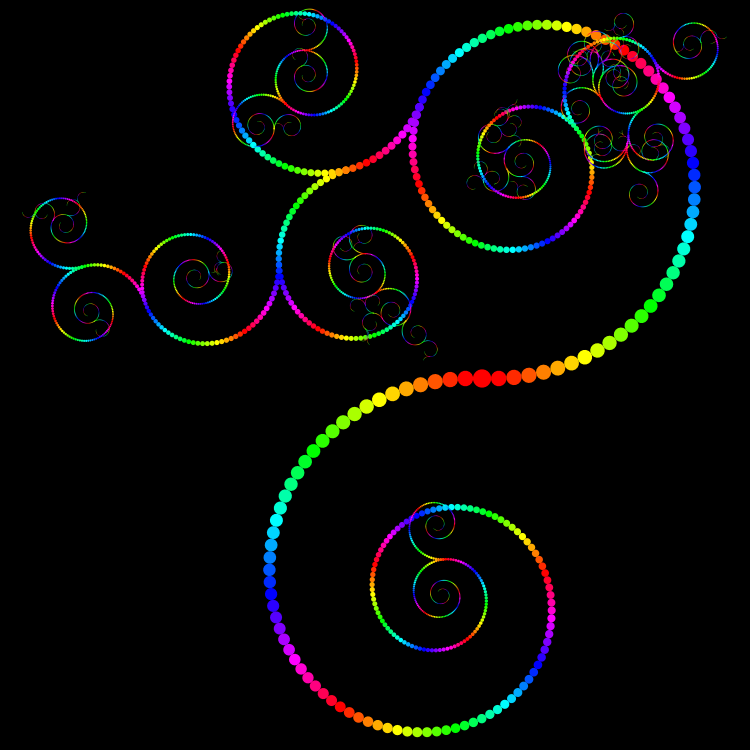
\includegraphics[width=\linewidth]{./images/exercise5.png}}
    \column{3cm}
    \fbox{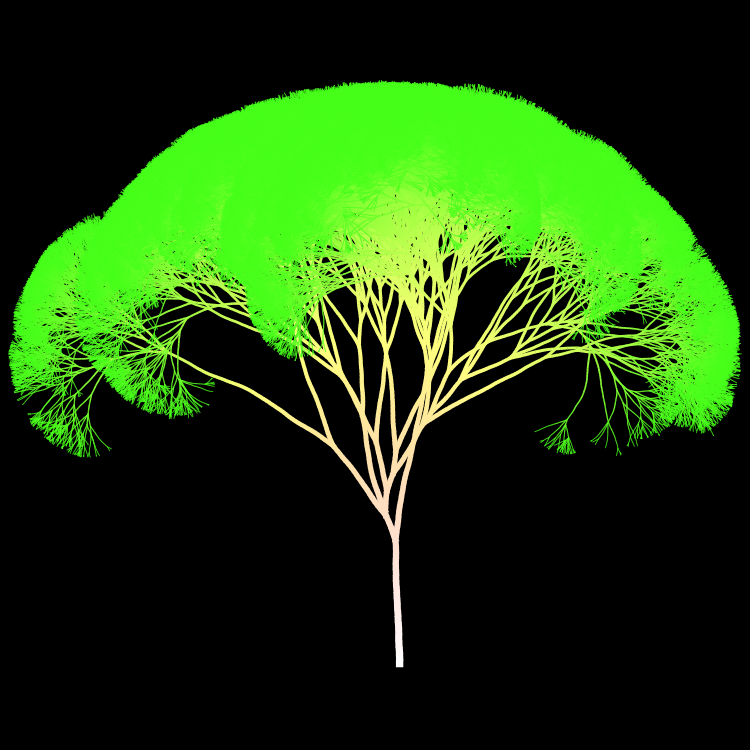
\includegraphics[width=\linewidth]{./images/exercise6.png}}
  \end{columns}
\end{frame}

\end{document}